%%%%%%%%%%%%%%%%%%%%%%%%%%%%%%%%%%%%%%%%%%%%%%%%%%%%%%%%%%%%%%%%%%%%%%%%%%%%%%%
%                       CARGA DE LA CLASE DE DOCUMENTO                        %
%%%%%%%%%%%%%%%%%%%%%%%%%%%%%%%%%%%%%%%%%%%%%%%%%%%%%%%%%%%%%%%%%%%%%%%%%%%%%%%

\documentclass[11pt,spanish,listoffigures,listoftables]{tfgetsinf}

%%%%%%%%%%%%%%%%%%%%%%%%%%%%%%%%%%%%%%%%%%%%%%%%%%%%%%%%%%%%%%%%%%%%%%%%%%%%%%%
%                          CODIFICACIÓN DEL FICHERO                           %
%%%%%%%%%%%%%%%%%%%%%%%%%%%%%%%%%%%%%%%%%%%%%%%%%%%%%%%%%%%%%%%%%%%%%%%%%%%%%%%

\usepackage[utf8]{inputenc} 
\usepackage{babel}
\usepackage{hyperref}
\usepackage{biblatex}
\usepackage{amsmath, amssymb}
\usepackage{graphicx}
\usepackage{booktabs}
\usepackage{listings}
\usepackage{xcolor}
\usepackage{multirow}
\usepackage{subcaption}

 

\addbibresource{bib.bib}  % Enlazar el archivo .bib
\addglobalbib{bib.bib}
\hypersetup{ colorlinks=true, linkcolor=black, urlcolor=cyan }

%%%%%%%%%%%%%%%%%%%%%%%%%%%%%%%%%%%%%%%%%%%%%%%%%%%%%%%%%%%%%%%%%%%%%%%%%%%%%%%
%                             OTROS PAQUETES                                  %
%%%%%%%%%%%%%%%%%%%%%%%%%%%%%%%%%%%%%%%%%%%%%%%%%%%%%%%%%%%%%%%%%%%%%%%%%%%%%%%
% (Aquí puedes añadir los paquetes que necesites)

%%%%%%%%%%%%%%%%%%%%%%%%%%%%%%%%%%%%%%%%%%%%%%%%%%%%%%%%%%%%%%%%%%%%%%%%%%%%%%%
%                         DATOS DEL TRABAJO                                   %
%%%%%%%%%%%%%%%%%%%%%%%%%%%%%%%%%%%%%%%%%%%%%%%%%%%%%%%%%%%%%%%%%%%%%%%%%%%%%%%

\title{Clasificación automática de artrosis en rodillas mediante redes neuronales convolucionales}
\author{Hernández Martínez, Carlos}
\tutor{Juan Ciscar, Alfonso}
\curs{2024-2025}

%%%%%%%%%%%%%%%%%%%%%%%%%%%%%%%%%%%%%%%%%%%%%%%%%%%%%%%%%%%%%%%%%%%%%%%%%%%%%%%
%            PALABRAS CLAVE Y RESÚMENES (en tres idiomas)                     %
%%%%%%%%%%%%%%%%%%%%%%%%%%%%%%%%%%%%%%%%%%%%%%%%%%%%%%%%%%%%%%%%%%%%%%%%%%%%%%%

\keywords{Palabras clave en catalán} % catalán
         {Palabras clave en español} % español
         {Keywords in English}       % inglés

% Añade esto en el preámbulo (antes de \begin{document})
\setcounter{tocdepth}{1} % Muestra solo capítulos y secciones en el índice
\begin{document}

%%%%%%%%%%%%%%%%%%%%%%%%%%%%%%%%%%%%%%%%%%%%%%%%%%%%%%%%%%%%%%%%%%%%%%%%%%%%%%%
%                             RESÚMENES                                       %
%%%%%%%%%%%%%%%%%%%%%%%%%%%%%%%%%%%%%%%%%%%%%%%%%%%%%%%%%%%%%%%%%%%%%%%%%%%%%%%

\begin{abstract}
Aquí citamos a un datajkjkset \cite{gornale2020digital}.
Citación paper IEE \cite{10863523}, Dataset \cite{chen2018knee}
aqui citamos un paper \cite{VAATTOVAARA2025100580}
otra cita \cite{comprehensive_review}

Quitar imagenes brillantes -> \cite{efficientnet_paper}
\end{abstract}

\begin{abstract}[spanish]
(Resumen en castellano)
\end{abstract}

\begin{abstract}[english]
(Resumen en inglés)
\end{abstract}

\mainmatter

%%%%%%%%%%%%%%%%%%%%%%%%%%%%%%%%%%%%%%%%%%%%%%%%%%%%%%%%%%%%%%%%%%%%%%%%%%%%%%%
%                              CAPÍTULO 1                                     %
%                                    INTRO                                     %
%%%%%%%%%%%%%%%%%%%%%%%%%%%%%%%%%%%%%%%%%%%%%%%%%%%%%%%%%%%%%%%%%%%%%%%%%%%%%%%

\chapter{Introducción}  % ~5 páginas

\section{Motivación}     % 1.1
La artritis es una de las enfermedades musculoesqueléticas más prevalentes a nivel mundial y una de las principales causas de discapacidad en adultos mayores. Su diagnóstico y seguimiento se basa tradicionalmente en la evaluación clínica y en la interpretación de imágenes médicas, como radiografías, resonancias magnéticas y tomografías computarizadas. Sin embargo, este proceso suele depender en gran medida de la experiencia del profesional médico, lo que puede generar variabilidad en los diagnósticos y retrasos en la detección temprana de la enfermedad.

En los últimos años, los avances en inteligencia artificial, y en particular en el aprendizaje profundo, han demostrado un gran potencial para mejorar la precisión y la eficiencia en el análisis de imágenes médicas. Las redes neuronales convolucionales (CNN) han sido ampliamente utilizadas en el campo de la visión por computadora para tareas como la detección de patologías en radiografías, la segmentación de tejidos en resonancias magnéticas y la clasificación de niveles de severidad en enfermedades degenerativas.

Este Trabajo de Fin de Grado (TFG) se motiva por la necesidad de desarrollar métodos automáticos y robustos para el análisis de la artritis mediante el uso de técnicas de aprendizaje profundo. En particular, se busca explorar el uso de redes neuronales para la clasificación de imágenes médicas, utilizando bases de datos estandarizadas como \textit{Mendeley dataset} \cite{chen2018knee}. La aplicación de estos modelos podría no solo optimizar el proceso de diagnóstico, sino también contribuir al desarrollo de herramientas de soporte a la decisión clínica, facilitando una intervención más temprana y personalizada para los pacientes.

La relevancia de este estudio radica en su potencial impacto en la práctica clínica. Un sistema basado en inteligencia artificial podría reducir la carga de trabajo de los especialistas, mejorar la objetividad del diagnóstico y ofrecer segundas opiniones automáticas que complementen la evaluación médica tradicional. Además, el desarrollo de estas tecnologías en el ámbito de la artritis podría sentar un precedente para su aplicación en otras enfermedades musculoesqueléticas, ampliando el alcance del aprendizaje profundo en el campo de la salud.

Además, se plantea la posibilidad de realizar \textit{transfer learning} utilizando modelos preentrenados en artritis humana para aplicarlos en el diagnóstico de artritis en gatos. Esta adaptación podría beneficiar la práctica veterinaria, proporcionando herramientas automatizadas para la evaluación de la enfermedad en animales y mejorando la precisión en su diagnóstico.

En este contexto, el presente trabajo busca contribuir al avance del uso de inteligencia artificial en la detección y análisis de la artritis, evaluando diferentes enfoques de redes neuronales y analizando su rendimiento en la clasificación de imágenes médicas. La motivación principal es demostrar la viabilidad y efectividad de estos modelos en un problema biomédico concreto, promoviendo la integración de tecnologías emergentes en el ámbito de la salud.


\section{Objetivos}      % 1.2
% Presenta aquí los 3 objetivos principales
% p.e. Objetivo 1, Objetivo 2, Objetivo 3

\section{Estructura del documento}  % 1.3
% Describe la organización de los capítulos y secciones

%%%%%%%%%%%%%%%%%%%%%%%%%%%%%%%%%%%%%%%%%%%%%%%%%%%%%%%%%%%%%%%%%%%%%%%%%%%%%%%
%                              CAPÍTULO 2                                     %
%                                PRELIMINARES (STANDBY)                       %
%%%%%%%%%%%%%%%%%%%%%%%%%%%%%%%%%%%%%%%%%%%%%%%%%%%%%%%%%%%%%%%%%%%%%%%%%%%%%%%

\chapter{Preliminares}  % ~15 páginas
\section{Aprendizaje automático}
El \textbf{aprendizaje automático} es una rama de la inteligencia artificial que se enfoca en que las máquinas mejoren 
su desempeño en una tarea determinada a partir de la experiencia \cite{Mitchell1997}. Un sistema \textit{“aprende”} cuando su desempeño en una tarea, 
medido por una métrica, mejora con la experiencia adquirida. En términos prácticos, esto implica diseñar algoritmos capaces de 
\textit{generalizar} patrones a partir de datos, de forma que puedan hacer predicciones o tomar decisiones sobre datos no vistos 
previamente. En aprendizaje automático se suelen representar los datos con un conjunto de \textit{características} (features) relevantes, y el algoritmo 
construye un modelo matemático que relaciona estas características con las salidas esperadas. Un objetivo central es lograr un buen 
equilibrio entre \textit{ajuste} a los datos de entrenamiento y \textit{capacidad de generalización} a nuevos datos, evitando problemas 
como el \textit{sobreajuste} (overfitting) \cite{Goodfellow2016}. La Figura~\ref{fig:overfitting} ilustra de forma visual las diferencias entre 
subajuste, buen ajuste y sobreajuste en un modelo supervisado, conceptos fundamentales para entender el rendimiento de los modelos de aprendizaje automático.

\begin{figure}[ht]
    \centering
    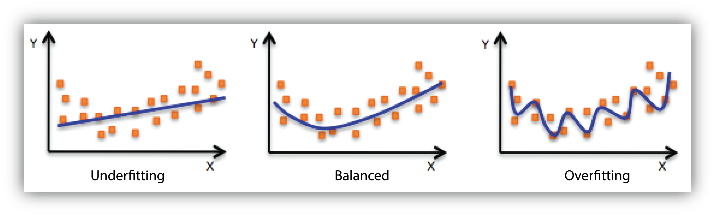
\includegraphics[width=0.7\textwidth]{under-overfitting.png}
    \caption{Ejemplo ilustrativo de subajuste, buen ajuste y sobreajuste en un modelo supervisado. Adaptado de \cite{awsOverfitting}.}
    \label{fig:overfitting}
\end{figure}

Existen varias categorías principales de aprendizaje automático, diferenciadas por la forma en que el algoritmo recibe la información 
y el tipo de tarea a resolver:
\begin{itemize}
    \item \textbf{Aprendizaje supervisado}: El algoritmo recibe ejemplos de entrada y su correspondiente salida deseada (etiquetas). 
    El objetivo es aprender una función que mapee las entradas a las salidas correctas. Son tareas típicas la \textit{clasificación} 
    (p. ej., dado un conjunto de características de un paciente, predecir si tiene una enfermedad: salida categórica) y la 
    \textit{regresión} (p. ej., predecir un valor numérico como el precio de una casa). El rendimiento se evalúa comúnmente con métricas
    como la exactitud en clasificación o el error cuadrático medio en regresión.

    \item \textbf{Aprendizaje no supervisado}: El algoritmo recibe datos de entrada sin etiquetas, y debe descubrir estructura oculta en 
    ellos. Incluye tareas como la \textit{clustering} (agrupamiento de datos por similitud) o la \textit{reducción de dimensionalidad} 
    (encontrar representaciones más compactas de los datos). Por ejemplo, un algoritmo no supervisado podría agrupar automáticamente 
    imágenes médicas en tipos similares sin conocer de antemano las patologías presentes.
    
    \item \textbf{Aprendizaje por refuerzo}: El algoritmo (un \textit{agente}) aprende a través de la interacción con un entorno, 
    recibiendo recompensas o penalizaciones según sus acciones. El agente debe descubrir una política de acciones que maximice la 
    recompensa acumulada. Este paradigma es común en robótica y juegos, donde no se proporcionan ejemplos de solución directa sino una 
    señal de calidad de cada acción.
    
\end{itemize}

El proceso típico de \textbf{aprendizaje supervisado} consiste en entrenar un modelo ajustando sus parámetros para minimizar un 
\textit{funcional de coste}, que mide el error de las predicciones del modelo sobre los datos de entrenamiento. El procedimiento de 
optimización más utilizado es el \textit{descenso de gradiente} y sus variantes, como el descenso de gradiente estocástico, que permite 
procesar los datos por lotes. En cada iteración, se calcula la gradiente del error respecto a los parámetros del modelo, y se ajustan los 
parámetros en la dirección opuesta a dicha gradiente para reducir el error. Este ciclo se repite múltiples veces (\textit{épocas}) 
hasta converger a un mínimo local del error.

La Figura~\ref{fig:gd_flow} muestra esquemáticamente el flujo de este proceso, desde la entrada de los datos hasta la actualización 
de los parámetros. A continuación, el Algoritmo~\ref{alg:gd-train} detalla los pasos fundamentales que se siguen durante el entrenamiento 
de un modelo mediante esta técnica.

\begin{figure}[ht]
    \centering
    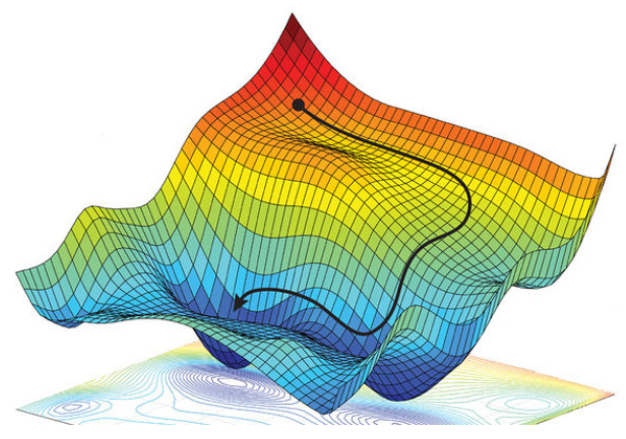
\includegraphics[width=0.8\textwidth]{descenso_gradiente.png}
    \caption{Flujo de entrenamiento de un modelo supervisado mediante descenso de gradiente. Adaptado de \cite{logongasBackprop}.}
    \label{fig:gd_flow}
\end{figure}

\begin{algorithmic}
    \label{alg:gd-train}
    \REQUIRE Conjunto de entrenamiento ${(x_i, y_i)}_{i=1}^N$, tasa de aprendizaje $\eta$ función de error $\mathcal{L}$
    \STATE Inicializar parámetros del modelo $\theta$ (p. ej. aleatoriamente)
    \FOR{numero de épocas}
        \FOR{cada $(x_i, y_i)$ en ${(x_i, y_i)}_{i=1}^N$}
            \STATE calcular predicción $\hat{y}_i = f_\theta(x_i)$
            \STATE calcular pérdida $L = \mathcal{L}(\hat{y}_i, y_i)$ \COMMENT{ej.: error cuadrático, entropía cruzada, etc.}
            \STATE calcular gradiente $g = \nabla_{\theta} L$
            \STATE actualizar parámetros: $\theta := \theta - \eta \cdot g$
        \ENDFOR
    \ENDFOR
\end{algorithmic}

Tras el entrenamiento, es fundamental evaluar el modelo con datos independientes (conjunto de \textit{prueba}) para estimar su capacidad de generalización. 
Además, suelen emplearse técnicas como \textit{validación cruzada} y conjuntos de \textit{validación} para ajustar hiperparámetros (parámetros del algoritmo 
que no se aprenden directamente, como la profundidad de un árbol de decisión o la tasa de aprendizaje $\eta$). Un buen enfoque de validación ayuda a prevenir 
el sobreajuste y a seleccionar modelos más robustos.

Existen algoritmos clásicos de AA como los \textit{árboles de decisión}, \textit{máquinas de vector soporte} (SVM), \textit{vecinos más cercanos} (k-NN), entre otros,
cada uno con sus supuestos y ámbitos de aplicación. Por ejemplo, las SVM buscan hiperplanos que separen clases maximizando el margen, mientras que los árboles de 
decisión realizan particiones recursivas del espacio de características para homogeneizar las etiquetas en los nodos hoja. La elección del algoritmo adecuado depende 
de la naturaleza de los datos y del problema a resolver, no existiendo un modelo único que sea óptimo para todas las tareas (teorema \textit{no free lunch}). Para 
profundizar en los fundamentos teóricos y prácticos del aprendizaje automático, se recomienda la literatura especializada, como los libros de Mitchell \cite{Mitchell1997} 
y Bishop \cite{Bishop2006}, que proporcionan una introducción comprensible y a la vez rigurosa al campo.

En resumen, el aprendizaje automático proporciona las bases para construir modelos que extraen conocimiento de los datos. Estos conceptos preliminares resultan 
imprescindibles para entender técnicas más avanzadas como las redes neuronales profundas y su aplicación en tareas de visión por computador y medicina, que se 
abordan en secciones posteriores.

\section{Redes Neuronales}\label{sec:nn} 

Las \textbf{redes neuronales artificiales} (RNA) constituyen una familia de modelos de aprendizaje automático inspirados vagamente en el cerebro humano. 
La unidad básica de una RNA es la \textit{neurona artificial}, un elemento que realiza una operación sencilla: calcula una combinación lineal de sus entradas y 
le aplica una función no lineal llamada \textit{función de activación}. Matemáticamente, si una neurona recibe como entradas $x_1, x_2, \dots, x_n$ con pesos 
sinápticos $w_1, w_2, \dots, w_n$ y tiene un sesgo $b$, produce una salida $y = \sigma(w_1 x_1 + w_2 x_2 + \cdots + w_n x_n + b)$, donde $\sigma(\cdot)$ podría ser, 
por ejemplo, una función sigmoide, tangente hiperbólica o ReLU (Unidad Lineal Rectificada). Las primeras RNA, como el \textit{Perceptrón} de Rosenblatt \cite{Rosenblatt1958},  tenían una 
sola capa de neuronas (una capa de entrada proyectada directamente a una capa de salida) y podían aprender a clasificar datos que fueran linealmente separables. 
Sin embargo, se demostró que una sola neurona (o capa lineal) tiene limitaciones significativas en su capacidad de representación.

La potencia de las redes neuronales radica en su capacidad para formar \textbf{arquitecturas multicapa}, también conocidas como \textit{redes neuronales de múltiples capas} 
o \textit{perceptrones multicapa} (MLP). Estas redes están organizadas en capas: una capa de entrada (los datos originales), una o varias capas \textit{ocultas} que 
realizan transformaciones intermedias mediante neuronas con sus pesos, y una capa de salida que produce la predicción final. Al agregar capas ocultas con funciones de 
activación no lineales, las redes adquieren la habilidad de aproximar relaciones no lineales arbitrariamente complejas entre la entrada y la salida (teorema de 
aproximación universal). 

\begin{figure}[htbp]
    \centering
    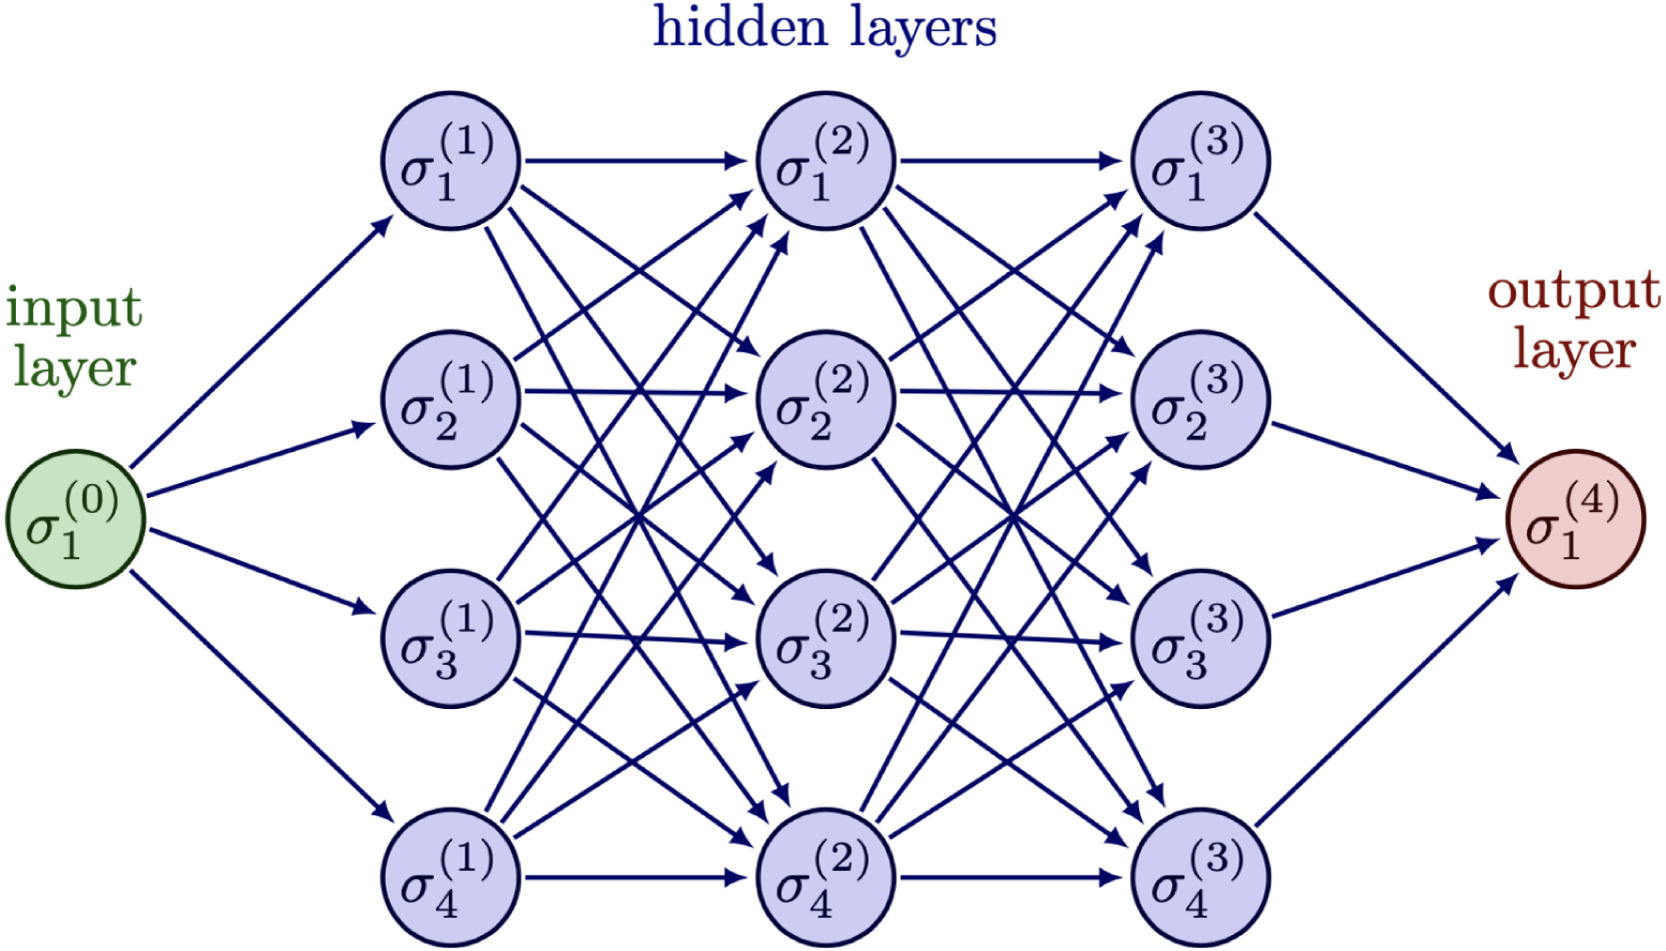
\includegraphics[width=0.5\textwidth]{neural_network.jpg}
    \caption{Ejemplo de una red neuronal profunda \cite{neural_network}}
    \label{fig:mi_imagen}
\end{figure}


El entrenamiento de una red neuronal multicapa se realiza típicamente mediante el algoritmo de \textit{retropropagación del error} (backpropagation) combinado con 
descenso de gradiente. En esencia, el procedimiento es: se calculan las salidas de la red para una entrada dada (\textit{fase forward}), se mide el error cometido 
comparando con la salida deseada mediante una función de coste (por ejemplo, la entropía cruzada para clasificación), y luego se propaga ese error hacia atrás a 
través de la red (\textit{fase backward}) calculando las derivadas parciales del error con respecto a cada peso utilizando la regla de la cadena. Estas derivadas 
indican cómo ajustar cada peso para reducir el error, y se aplican las actualizaciones de los pesos en consecuencia. Gracias a la retropropagación, las redes neuronales 
pueden entrenarse eficientemente incluso con muchas capas, ajustando millones de parámetros para adaptarse a complejos conjuntos de datos. Este avance fue crucial para 
el renacimiento de las redes neuronales en la década de 1980, tras un período de estancamiento parcial debido a las limitaciones de los perceptrones simples destacadas 
por Minsky y Papert en 1969 (quienes señalaron, por ejemplo, que un perceptrón no podía aprender la función XOR). El trabajo de Rumelhart, Hinton y Williams (1986) \cite{Rumelhart1986}
introdujo formalmente la retropropagación, mostrando que las redes de múltiples capas podían aprender características jerárquicas y superar esas limitaciones previas.

A medida que se dispuso de más datos y mayor potencia de cómputo, especialmente con la llegada de unidades de procesamiento gráfico (GPU) que aceleraron el cálculo 
matricial masivo, las redes neuronales crecieron en profundidad y capacidad. Surge así el campo del \textbf{aprendizaje profundo} (\textit{deep learning}), que no es 
más que el uso de redes neuronales con muchas capas (a veces decenas o incluso cientos) entrenadas sobre grandes volúmenes de datos. Un hito simbólico fue la competición 
ImageNet de 2012, en la cual una red convolucional profunda llamada \textit{AlexNet} \cite{Krizhevsky2012} obtuvo un rendimiento muy superior al de los métodos tradicionales en la tarea de 
clasificación de imágenes a gran escala. AlexNet, desarrollada por Krizhevsky et al. (2012), tenía 8 capas entrenables y introdujo técnicas como capas de \textit{dropout} 
para regularización y entrenamiento en GPU, marcando el inicio de una nueva era en visión por computador impulsada por redes neuronales profundas. Desde entonces, 
arquitecturas aún más profundas y sofisticadas han emergido, como \textit{VGGNet} (2014, 16-19 capas), \textit{Inception/GoogLeNet} (2015, con módulos de convolución 
en paralelo) y \textit{ResNet} \cite{He2016} (2016, más de 50 capas). En particular, las \textbf{redes residuales} (ResNets) de He et al. (2016) introdujeron conexiones de atajo 
(skip connections) que mitigaron el problema de la degradación del gradiente en redes muy profundas, permitiendo entrenar exitosamente redes de incluso 152 capas con 
mejoras significativas en la precisión de tareas de visión.

Una clase especial y sumamente importante de RNA para datos con estructura espacial o temporal son las \textbf{redes neuronales convolucionales} 
(CNN, por sus siglas en inglés). Las CNN fueron concebidas originalmente para procesar imágenes, inspiradas en la organización del córtex visual animal. 
En una CNN, en lugar de conectar todas las neuronas de una capa a todas las de la siguiente (como en un MLP denso tradicional), se emplean \textit{capas convolucionales} 
donde cada neurona está conectada solo a una región local de la capa anterior (campo receptivo) y todos los neuronas de una capa comparten conjuntos de pesos (filtros)
que se \textit{desplazan} sobre la entrada. Esta estructura explota las propiedades de \textit{estacionaridad} de las imágenes (patrones locales similares pueden 
aparecer en cualquier ubicación) y reduce drásticamente el número de parámetros al introducir \textit{pesos compartidos}. Además, se intercalan típicamente 
\textit{capas de pooling} (submuestreo), que reducen la resolución espacial agrupando activaciones cercanas (por ejemplo, tomando el máximo de cada bloque $2\times2$ 
de neuronas), confiriendo invarianza a traslaciones pequeñas y reduciendo la dimensionalidad progresivamente. Una arquitectura CNN típica para clasificación de 
imágenes consiste en varias capas convolucionales+pooling en cascada, que extraen características cada vez más abstractas de la imagen (bordes, texturas, partes, objetos), 
seguidas de una o más capas totalmente conectadas que actúan como clasificador final sobre esas características extraídas. La Figura \ref{fig:cnn_arch} muestra 
esquemáticamente un ejemplo de arquitectura CNN simple, con sus etapas de convolución, pooling y capas densas finales.

\begin{figure}[ht] \centering 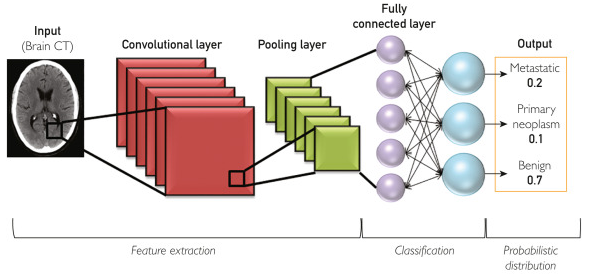
\includegraphics[width=0.8\textwidth]{cnn.png} 
    \caption{Ejemplo de arquitectura de una red neuronal convolucional para clasificación de imágenes. Se observan capas convolucionales (conv) que aplican 
    filtros aprendibles sobre la imagen de entrada, seguidas de capas de pooling que reducen la resolución. Al final, capas totalmente conectadas (FC) procesan 
    las características extraídas para producir la clasificación en alguna de las categorías.} 
    \label{fig:cnn_arch} 
\end{figure}

Las CNN han demostrado ser extremadamente efectivas en visión por computador, logrando reconocer objetos en fotos con gran precisión, segmentar imágenes píxel a píxel, 
detectar rostros, entre muchas otras aplicaciones. En el ámbito de imágenes médicas, han superado enfoques tradicionales al detectar patrones sutiles en radiografías, 
resonancias o microscopías que serían difíciles de modelar manualmente. No obstante, entrenar redes profundas con éxito requiere prácticas adecuadas: grandes conjuntos 
de datos anotados, técnicas de regularización (como \textit{dropout}, normalización batch, data augmentation), y a menudo un ajuste cuidadoso de hiperparámetros. 
Cuando el conjunto de datos disponible es limitado (situación común en aplicaciones biomédicas), es frecuente recurrir a \textit{aprendizaje por transferencia}, 
utilizando redes pre-entrenadas en un dominio amplio (p. ej., ImageNet) y refinándolas (fine-tuning) sobre la tarea específica, aprovechando características visuales 
genéricas aprendidas previamente.

Otro aspecto relevante es la \textit{interpretabilidad} de las predicciones de las redes neuronales. Las RNA profundas han sido criticadas como “cajas negras” 
difíciles de entender; sin embargo, se han desarrollado técnicas para visualizar y explicar qué han aprendido. Por ejemplo, en imágenes, métodos como \textit{Grad-CAM} 
(Gradiente-Weighted Class Activation Mapping) \cite{vanDerVelden2022} permiten resaltar las regiones de la imagen que más contribuyen a una determinada predicción de la red, proporcionando 
pistas sobre qué está “mirando” la CNN al tomar su decisión. Estas técnicas forman parte de la llamada \textbf{IA explicable} (XAI, \textit{Explainable AI}), 
un campo emergente que busca hacer más transparente el funcionamiento de modelos complejos, especialmente crítico en entornos como la medicina donde es necesario ganar 
la confianza del especialista humano.

En suma, las redes neuronales (especialmente las convolucionales profundas) constituyen la columna vertebral de muchos sistemas modernos de inteligencia artificial, 
logrando avances sin precedentes en reconocimiento de patrones. Para una cobertura más amplia sobre arquitecturas y fundamentos de aprendizaje profundo, puede 
consultarse el texto de Goodfellow et al. En la siguiente sección se explorará cómo estas técnicas de AA y redes neuronales se aplican en el ámbito de la visión por 
computador biomédica, con énfasis en el caso concreto de la clasificación de artrosis de rodilla mediante CNN.

\section{ML aplicado a VC y tareas biomédicas: caso MedMNIST}\label{sec:ml-medical} 
La combinación de aprendizaje automático y visión por computador ha impulsado grandes avances en el análisis de imágenes biomédicas 
en la última década. En el pasado, la interpretación de imágenes médicas (radiografías, resonancias, microscopia, etc.) dependía 
enteramente de la pericia humana, pero hoy en día los algoritmos de \textit{deep learning} han logrado igualar e incluso superar 
el rendimiento de expertos en ciertas tareas diagnósticas \cite{Liu2019}. Por ejemplo, se han entrenado redes neuronales convolucionales para 
detectar retinopatía diabética en fotos de retina, cáncer de piel en imágenes dermatoscópicas, neumonía en radiografías de tórax, 
entre otros, con niveles de sensibilidad y especificidad comparables a los de médicos especialistas. Un metaanálisis de Liu et al. 
(2019) recopiló numerosos estudios y concluyó que los clasificadores basados en aprendizaje profundo tenían, en promedio, un 
desempeño similar al de profesionales de la salud en la detección de enfermedades a partir de imágenes médicas, lo que subraya el 
potencial de estas técnicas para apoyar la labor clínica.

En el caso particular de la \textbf{artrosis de rodilla} (u osteoartritis), la radiografía es la técnica más utilizada para evaluar 
la gravedad de la enfermedad. Los radiólogos emplean un criterio estandarizado, la \textit{escala Kellgren-Lawrence (KL)} \cite{kellgren_lawrence_radiopaedia}, que asigna 
un grado de 0 a 4 a la rodilla en función de signos radiográficos de degeneración (osteofitos, estrechamiento del espacio articular, 
esclerosis, deformidad). Sin embargo, la lectura de estas radiografías puede ser subjetiva y presentar variabilidad entre observadores.
Por ello, existe un gran interés en desarrollar sistemas automáticos que clasifiquen el grado KL a partir de la imagen de rayos X de 
la rodilla de forma consistente y reproducible. Las redes neuronales convolucionales se adaptan muy bien a este problema: pueden 
entrenarse con conjuntos grandes de radiografías anotadas con su grado KL para aprender directamente las características visuales 
asociadas \cite{Rani2024} a cada nivel de severidad.

Dado el amplio espectro de modalidades y problemas en imágenes médicas, han surgido iniciativas para facilitar la investigación 
y comparación de algoritmos en múltiples tareas. Un caso notable es \textbf{MedMNIST} \cite{Yang2022}, una colección de datasets biomédicos de 
pequeño tamaño inspirada en el famoso MNIST (dataset de dígitos escritos a mano) pero orientada a imágenes médicas . MedMNIST, en 
su versión más reciente \textit{MedMNIST v2}, recopila 12 conjuntos de datos 2D (imágenes estáticas de 28$\times$28 píxeles) y 6 
conjuntos 3D (volúmenes de 28$\times$28$\times$28 voxeles), abarcando diversas modalidades y tareas de clasificación biomédica. 
Por ejemplo, incluye desde láminas histológicas coloreadas (\textit{PathMNIST}, 9 clases de tejidos patológicos), imágenes 
dermatoscópicas de lunares (\textit{DermaMNIST}, clasificación de lesiones cutáneas), y radiografías de tórax 
(\textit{ChestMNIST}, etiquetas multilabel de hallazgos torácicos), hasta estudios de retina OCT (\textit{OCTMNIST}, detección 
de patologías retinales), entre otros. Cada subconjunto viene ya preprocesado y separado en particiones de entrenamiento, 
validación y prueba estandarizadas, lo que facilita la aplicación directa de algoritmos y la comparación justa entre ellos.

MedMNIST \cite{Yang2022} fue diseñado con varios objetivos clave en mente:
\begin{itemize}
    \item \textbf{Diversidad}: Cubre múltiples modalidades de imagen (radiografías, tomografías, resonancias, ecografías, 
    imágenes microscopias, etc.), distintos tamaños de datos (desde $\sim$100 hasta $>$100,000 imágenes) y tareas de 
    clasificación variadas (binaria, multiclase, multietiqueta e incluso regresión ordinal). Esto permite evaluar la generalización 
    de los algoritmos de aprendizaje automático en distintos escenarios con un solo recurso unificado.
    
    \item \textbf{Estandarización}: Todos los conjuntos están uniformizados a la misma resolución (imágenes pequeñas de $28\times28$ 
    pixeles para 2D, o cubos de $28^3$ para 3D) con formato de datos consistente. Asimismo, se proveen divisiones oficiales en 
    entrenamiento/validación/test para cada dataset. Gracias a esto, los investigadores pueden centrarse en diseñar y probar 
    modelos de \textit{machine learning} sin preocuparse por el preprocesamiento de datos o posibles sesgos en la separación 
    de conjuntos, y los resultados son comparables entre diferentes estudios de forma más directa.
    
    \item \textbf{Ligereza y accesibilidad}:  El reducido tamaño de las imágenes hace que ejecutar experimentos sea computacionalmente 
    liviano, incluso sin hardware especializado. Además, la colección es de libre acceso con licencia abierta (CC BY) y cuenta con una 
    API unificada (disponible vía \texttt{pip install medmnist}) para cargar los datos fácilmente en diversos lenguajes. 
    Esto democratiza la experimentación en análisis de imágenes médicas, permitiendo a estudiantes y grupos con recursos limitados 
    explorar algoritmos de clasificación sobre datos reales de medicina.

    \item \textbf{Benchmark}: MedMNIST sirve tanto para introducir a nuevos usuarios en el campo de la visión médica, al 
    proporcionar casos ya preparados sobre los cuales practicar, como para benchmarking de algoritmos de AutoML y redes 
    neuronales en múltiples tareas livianas. Al enfocarse en imágenes pequeñas, enfatiza más el aspecto algorítmico 
    (diseño del modelo, estrategias de aprendizaje) que el meramente computacional. De hecho, trabajos asociados han 
    evaluado métodos clásicos de deep learning (ResNet, DenseNet, etc.) y herramientas AutoML sobre MedMNIST, generando 
    un punto de referencia inicial de desempeños.
\end{itemize}

En resumen, iniciativas como MedMNIST complementan a los grandes desafíos clínicos (ej. clasificar artrosis en radiografías 
completas) ofreciendo un “laboratorio” controlado para probar métodos de aprendizaje automático en imágenes biomédicas. 
El presente proyecto de TFG se enmarca precisamente en este contexto: la aplicación de redes neuronales convolucionales 
al diagnóstico automatizado de artrosis de rodilla, un problema relevante en el campo de la salud musculoesquelética. 
Aprovechando conjuntos de datos como el de OAI \cite{chen2018knee} (con imágenes reales de pacientes) y los avances reportados en la literatura, se 
buscará entrenar un modelo capaz de predecir el estado de la articulación a partir de la radiografía, evaluando su desempeño 
y explorando técnicas de interpretación (por ejemplo, visualizando las regiones de la rodilla más influyentes en la decisión 
de la red mediante mapas de calor al estilo Grad-CAM). De este modo, se pretende contribuir tanto a la validación de las 
técnicas de aprendizaje profundo en una tarea biomédica específica como a la comprensión de sus alcances y limitaciones en 
un entorno clínico real.


%%%%%%%%%%%%%%%%%%%%%%%%%%%%%%%%%%%%%%%%%%%%%%%%%%%%%%%%%%%%%%%%%%%%%%%%%%%%%%%
%                              CAPÍTULO 3                                     %
%                     DESCRIPCIÓN DEL CORPUS DEL DATASET OAI                 %
%%%%%%%%%%%%%%%%%%%%%%%%%%%%%%%%%%%%%%%%%%%%%%%%%%%%%%%%%%%%%%%%%%%%%%%%%%%%%%%


\chapter{Corpus del Dataset OAI y tareas comunes}
\label{chap:corpus}

\section{Introducción al dataset OAI}

El estudio de la artrosis de rodilla requiere de conjuntos de datos que reflejen con fidelidad tanto la progresión clínica 
como los cambios estructurales visibles en técnicas de imagen. En este contexto, el \textit{Osteoarthritis Initiative (OAI)}\cite{chen2018knee}
se posiciona como una de las bases de datos públicas más relevantes y ampliamente utilizadas en investigaciones biomédicas. 
Este repositorio fue concebido con el objetivo de identificar biomarcadores de progresión y aparición de la osteoartritis, 
facilitando el desarrollo de herramientas diagnósticas y terapéuticas más precisas.

El proyecto OAI comenzó en 2004 y ha recopilado datos longitudinales de aproximadamente 4.796 participantes durante más de una 
década. Los sujetos fueron seleccionados de diferentes centros médicos de Estados Unidos, e incluyen tanto individuos con 
diagnóstico clínico de artrosis como sujetos en riesgo de desarrollarla. Esta diversidad poblacional permite estudiar la 
evolución de la enfermedad desde fases asintomáticas hasta estadios avanzados.

Este conjunto de datos es especialmente valioso para tareas de aprendizaje automático debido a su tamaño, su naturaleza longitudinal y la inclusión de etiquetas clínicamente validadas. Asimismo, permite abordar problemas tanto de clasificación como de predicción de progresión de la enfermedad.

\begin{figure}[htbp]
    \centering
    \begin{subfigure}[b]{0.19\textwidth}
        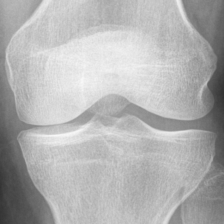
\includegraphics[width=\textwidth]{knee_0.png}
        \caption{KL 0}
        \label{fig:knee0}
    \end{subfigure}
    \hfill
    \begin{subfigure}[b]{0.19\textwidth}
        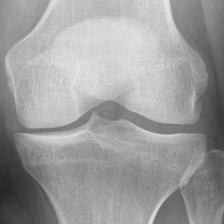
\includegraphics[width=\textwidth]{knee_1.png}
        \caption{KL 1}
        \label{fig:knee1}
    \end{subfigure}
    \hfill
    \begin{subfigure}[b]{0.19\textwidth}
        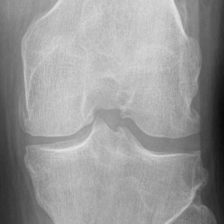
\includegraphics[width=\textwidth]{knee_2.png}
        \caption{KL 2}
        \label{fig:knee2}
    \end{subfigure}
    \hfill
    \begin{subfigure}[b]{0.19\textwidth}
        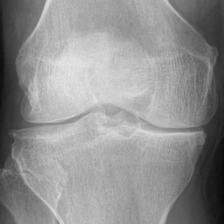
\includegraphics[width=\textwidth]{knee_3.png}
        \caption{KL 3}
        \label{fig:knee3}
    \end{subfigure}
    \hfill
    \begin{subfigure}[b]{0.19\textwidth}
        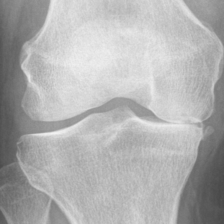
\includegraphics[width=\textwidth]{knee_4.png}
        \caption{KL 4}
        \label{fig:knee4}
    \end{subfigure}
    \caption{Ejemplos de radiografías de rodilla clasificadas según la escala Kellgren \& Lawrence (KL)}
    \label{fig:knee-examples}
\end{figure}



\section{--------Previo---------}
En este capítulo se presenta una descripción exhaustiva del corpus utilizado para la detección y gradación de la artrosis en rodillas. Se abordan aspectos fundamentales relativos al dataset OAI, obtenido de Mendeley Data, así como la integración de elementos experimentales extraídos del paper \cite{efficientnet_paper}. En este contexto, se detallan los procesos de adquisición, preprocesamiento, análisis estadístico y organización en subconjuntos, elementos esenciales para el éxito en la aplicación de modelos de aprendizaje profundo.

\section{Adquisición y Descripción del Dataset OAI}
El dataset OAI se obtuvo de la plataforma Mendeley Data y se ha consolidado como una fuente de referencia para el estudio de la artrosis de rodilla. Este corpus se compone de radiografías que permiten evaluar la severidad de la enfermedad mediante el sistema de gradación de Kellgren-Lawrence (KL). Durante la fase de adquisición se integraron las clases \textit{test}, \textit{train}, \textit{val} y \textit{auto-test} presentadas en el dataset original, logrando el split empleado en \cite{efficientnet_paper}. Concretamente, el conjunto se redistribuyó en un 75\% para entrenamiento, 17\% para prueba y 8\% para validación.

\subsection{Distribución por Condición Médica y Estadísticas del Corpus}
En este trabajo, las clases se denominan de acuerdo con la condición médica asociada a la artrosis:
\begin{itemize}
    \item \textbf{Sin artrosis} (KL 0)
    \item \textbf{Leve} (KL 1)
    \item \textbf{Moderada} (KL 2)
    \item \textbf{Severa} (KL 3)
    \item \textbf{Muy severa} (KL 4)
\end{itemize}

La siguiente tabla resume la distribución numérica de imágenes en cada subconjunto:
\begin{center}
\begin{tabular}{lccccc}
\toprule
\textbf{Subconjunto} & \textbf{Sin artrosis} & \textbf{Leve} & \textbf{Moderada} & \textbf{Severa} & \textbf{Muy severa} \\
\midrule
\textit{auto-test} & 604 & 275 & 403 & 200 & 44 \\
\textit{train}     & 2286 & 1046 & 1516 & 757 & 173 \\
\textit{val}       & 328 & 153 & 212 & 106 & 27 \\
\textit{test}      & 639 & 296 & 447 & 223 & 51 \\
\bottomrule
\end{tabular}
\end{center}

Como complemento, se detallan a continuación los porcentajes de distribución por clase en cada
 subconjunto:

Conjunto de datos por clase
\begin{itemize}
    \item Sin artrosis: 39.5\%
    \item Leve: 18\%
    \item Moderada: 26.5\%
    \item Severa: 13\%
    \item Muy severa: 3\%
\end{itemize}
El corpus total se compone de 9786 imágenes, distribuidas en 1526 para auto-test, 5778 para entrenamiento, 826 para validación y 
1656 para prueba. Esta distribución y el equilibrio en las condiciones médicas son fundamentales para el entrenamiento y evaluación r
obusta de los modelos de clasificación.

\section{Preprocesamiento y Análisis del Corpus}
El preprocesamiento de las imágenes es una etapa crucial para asegurar la calidad y homogeneidad de los datos. Se aplicaron las siguientes técnicas:

\begin{itemize}
    \item \textbf{Redimensionamiento y Conversión a RGB:} Se ajustaron todas las imágenes a un tamaño uniforme de 224$\times$224 píxeles y se convirtieron al formato RGB, cumpliendo con las especificaciones de entrada de arquitecturas como EfficientNet.
    \item \textbf{Ecualización de Histograma:} Esta técnica se utilizó para mejorar el contraste, resaltando detalles fundamentales para la detección de patrones asociados a la artrosis.
    \item \textbf{Filtrado Bilateral:} Aplicado para suavizar las imágenes preservando bordes y detalles críticos, esenciales para la correcta interpretación anatómica.
    \item \textbf{Data Augmentation:} Se implementaron técnicas de aumento de datos (volteo horizontal y vertical) en el conjunto de entrenamiento, incrementando la variabilidad y robustez del modelo sin alterar la integridad de los conjuntos de validación y prueba.
\end{itemize}

El análisis estadístico del corpus resalta una distribución equilibrada entre las diferentes condiciones médicas, lo que es vital para el aprendizaje profundo y la posterior validación del modelo.

\section{Integración con el Paper}
El paper \cite{efficientnet_paper} utiliza el dataset OAI para evaluar un modelo ensemble basado en arquitecturas EfficientNet, mediante:

\begin{itemize}
    \item \textbf{Modelo Ensemble:} La combinación de EfficientNetB0 y EfficientNetB4 permite mejorar la precisión en la clasificación, aprovechando las fortalezas complementarias de cada arquitectura.
    \item \textbf{Estrategia de Entrenamiento:} Se han empleado pesos pre-entrenados junto con técnicas de regularización (Dropout y penalización L2) para optimizar la convergencia del modelo y minimizar el riesgo de sobreajuste.
    \item \textbf{Explainable AI:} La técnica Grad-CAM facilita la interpretación visual de las áreas críticas que influyen en las predicciones, aumentando la transparencia y confiabilidad del sistema.
\end{itemize}

La integración de estas metodologías, junto con el exhaustivo preprocesamiento y análisis del corpus, permite obtener resultados experimentales comparables con el estado del arte en la detección y gradación de la artrosis de rodilla.

\section{Conclusiones}
El análisis detallado del corpus del dataset OAI y su integración con las técnicas presentadas en \cite{efficientnet_paper} subraya la importancia de una adquisición y preprocesamiento minuciosos. La organización en subconjuntos, el equilibrio en la distribución de condiciones médicas y la aplicación de técnicas avanzadas en el tratamiento de imágenes sientan las bases para el desarrollo de modelos de aprendizaje profundo capaces de ofrecer diagnósticos precisos y fiables. Este enfoque contribuye significativamente al desarrollo de herramientas de asistencia al diagnóstico que combinan inteligencia artificial con técnicas de Explainable AI.

%%%%%%%%%%%%%%%%%%%%%%%%%%%%%%%%%%%%%%%%%%%%%%%%%%%%%%%%%%%%%%%%%%%%%%%%%%%%%%%


\chapter{Capítulo X | contribución 1: Experimentación y Análisis de Resultados}

\section{Introducción}
En este capítulo se presentan los experimentos realizados para evaluar el desempeño de diversas arquitecturas de redes neuronales en la detección de artrosis en rodillas. Con el objetivo de aportar evidencia empírica para la detección temprana de la enfermedad, se han probado variantes de modelos EfficientNet y ResNet utilizando dos estrategias de entrenamiento: el uso de pesos pre-entrenados (transfer learning) y el entrenamiento desde cero (\textit{from scratch}). Los experimentos se han llevado a cabo sobre el conjunto de datos Mendeley \cite{chen2018knee} y se han tomado como referencia las aportaciones teóricas y experimentales descritas en \cite{efficientnet_paper}. 

\section{Metodología Experimental}

\subsection{Configuración del Experimento}
Para todos los experimentos se siguió el siguiente protocolo:
\begin{itemize}
    \item \textbf{Preprocesamiento:} Se redimensionaron las imágenes a un tamaño uniforme (224x224), se aplicaron técnicas de histogram equalization y bilateral filtering y transformación de la imagen a RGB. Aparte de un aumentos de datos (flip horizontal y vertical) para mejorar la generalización del modelo.
    \item \textbf{Partición del Conjunto de Datos:} El dataset se dividió en subconjuntos de entrenamiento, validación y prueba, siguiendo los porcentajes previamente establecidos. 75\% para entrenamiento, 17\% para prueba y 8\% para validación.
    \item \textbf{Configuración de Entrenamiento:} Se usó la función de pérdida \textit{Categorical Cross-Entropy} y el optimizador Adam con una tasa de aprendizaje inicial de 0.001, aplicando un scheduler para la reducción de la tasa en caso de estancamiento. Se entrenó hasta 50 épocas, implementando técnicas de Early Stopping para evitar sobreajuste. También se aplicó regularización L2 con valores entre 0.001 y 0.0001 para prevenir el sobreajuste.
\end{itemize}

\subsection{Modelos Evaluados}
Se evaluaron las siguientes arquitecturas:
\begin{itemize}
    \item \textbf{EfficientNet:} De la familia se probaron los modelos B0, B4, B5 y B7
    \item \textbf{ResNet50:} Modelo representativo de la familia ResNet.
\end{itemize}

\subsection{Estrategias de Entrenamiento}
Se compararon dos enfoques:
\begin{enumerate}
    \item \textbf{Transfer Learning:} Utilizando pesos pre-entrenados en grandes bases de datos (por ejemplo, ImageNet) para adaptar el modelo a la tarea específica de clasificación de artrosis.
    \item \textbf{Entrenamiento Desde Cero (\textit{From Scratch}):} Inicializando los pesos de manera aleatoria y entrenando la red sin conocimiento previo.
\end{enumerate}

\section{Resultados Experimentales}

\subsection{Comparación de Arquitecturas y Estrategias}
Los experimentos demostraron que, en su mayoría, tanto los modelos EfficientNet como los ResNet alcanzaron precisiones cercanas al 70\%, excepto EfficientNetB5 que logró una precisión del 71\%. La Tabla \ref{tab:resultados_experimentos} resume los resultados obtenidos.
La precisión obtenida se escogió en base a la época de entrenamiento con menor pérdida. En algunos casos los modelos conseguian una mejor precisión con mayor perdida, pero no siendo significativa la mejora.
\begin{table}[htbp]
\centering
\begin{tabular}{lccc}
\toprule
\textbf{Modelo y Estrategia} & \textbf{Precisión (\%)} & \textbf{Val loss} & \textbf{Épocas necesarias} \\
\midrule
EfficientNetB0 (Pre-entrenado)  & 69.87\%    & 0.73 & 7 \\
EfficientNetB5 (Pre-entrenado)  & 72.82\%    & 0.81 & 2 \\
EfficientNetB7 (Pre-entrenado)  & 66.54\%    & 0.79 & 13 \\
EfficientNetB4 (Desde Cero)     & 59.36\%    & 0.96 & 49 \\
ResNet50 (Pre-entrenado)        & 66.66\%    & 0.78 & 4 \\
ResNet50 (Desde Cero)           & 65.89\%    & 0.84 & 28 \\

\bottomrule
\end{tabular}
\caption{Comparación de modelos y estrategias de entrenamiento}
\label{tab:resultados_experimentos}
\end{table}

\begin{figure}[htbp]
    \centering
    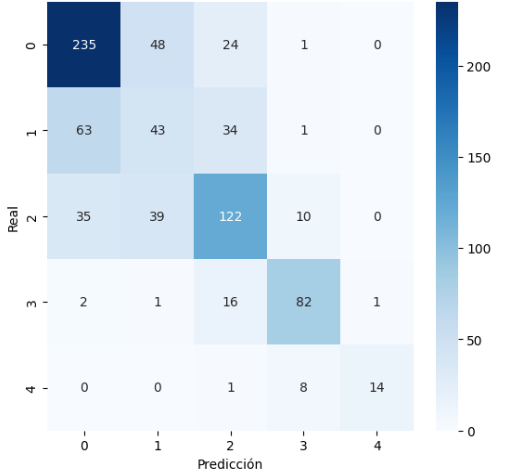
\includegraphics[width=0.6\textwidth]{EfficientNet_B7.png}
    \caption{Descripción de la imagen}
    \label{fig:matriz_confusion}
\end{figure}

\subsection{Impacto del Uso de Pesos Pre-entrenados}
Los experimentos evidenciaron que:
\begin{itemize}
    \item \textbf{Convergencia Rápida:} Los modelos con pesos pre-entrenados alcanzaron la convergencia en menos épocas, reduciendo significativamente el tiempo de entrenamiento.
    \item \textbf{Mayor Precisión:} Se observó un aumento en la precisión (hasta 71\% en el caso de EfficientNetB5) en comparación con el entrenamiento desde cero, donde los resultados se situaron en torno al 67-68\%.
    \item \textbf{Robustez del Modelo:} Los modelos pre-entrenados realizaban un overfitting mas pronunciado, pero la precisión obtenida era mayor que los modelos entrenados desde cero.
\end{itemize}

\subsection{Análisis Comparativo y Discusión}
La comparación entre los dos enfoques de entrenamiento resalta la importancia de la transferencia de aprendizaje en el dominio biomédico:
\begin{itemize}
    \item Aunque la mejora en precisión entre modelos pre-entrenados y entrenados desde cero es modesta (aproximadamente un 1-2\%), esta diferencia es crucial en aplicaciones clínicas, donde cada punto porcentual puede tener un impacto significativo en el diagnóstico.
    \item El entrenamiento desde cero presentó desventajas claras, tales como un mayor consumo de recursos computacionales y un tiempo de entrenamiento considerablemente más largo, lo cual puede ser prohibitivo en entornos con recursos limitados.
    \item EfficientNetB5 destacó frente a las demás arquitecturas, lo que sugiere que una mayor capacidad del modelo (a pesar de aumentar la complejidad) puede traducirse en mejoras en el desempeño, siempre y cuando se disponga de una estrategia de entrenamiento adecuada.
\end{itemize}

\section{Conclusiones del Capítulo}
Los experimentos realizados permiten concluir que:

\cleardoublepage


\chapter{Capítulo 2 de contribución}   % ~15 páginas
% Expón aquí tu segundo objetivo y resultados derivados

%%%%%%%%%%%%%%%%%%%%%%%%%%%%%%%%%%%%%%%%%%%%%%%%%%%%%%%%%%%%%%%%%%%%%%%%%%%%%%%
%                              CAPÍTULO 5                                     %
%                     TERCERA CONTRIBUCIÓN (OBJETIVO 3)                       %
%%%%%%%%%%%%%%%%%%%%%%%%%%%%%%%%%%%%%%%%%%%%%%%%%%%%%%%%%%%%%%%%%%%%%%%%%%%%%%%

\chapter{Capítulo 3 de contribución}   % ~15 páginas
% Expón aquí tu tercer objetivo y resultados derivados

%%%%%%%%%%%%%%%%%%%%%%%%%%%%%%%%%%%%%%%%%%%%%%%%%%%%%%%%%%%%%%%%%%%%%%%%%%%%%%%
%                              CAPÍTULO 6                                     %
%                                CONCLUSIONES                                 %
%%%%%%%%%%%%%%%%%%%%%%%%%%%%%%%%%%%%%%%%%%%%%%%%%%%%%%%%%%%%%%%%%%%%%%%%%%%%%%%

\chapter{Conclusiones}  % ~5 páginas

\section{Resumen del trabajo realizado} % 6.1
% Repasa y sintetiza las secciones principales

\section{Objetivos alcanzados}         % 6.2
% Verifica si se cumplieron los objetivos planteados

\section{Trabajo futuro}               % 6.3
% Explica las posibles extensiones o mejoras

%%%%%%%%%%%%%%%%%%%%%%%%%%%%%%%%%%%%%%%%%%%%%%%%%%%%%%%%%%%%%%%%%%%%%%%%%%%%%%%
%                              BIBLIOGRAFÍA                                   %
%%%%%%%%%%%%%%%%%%%%%%%%%%%%%%%%%%%%%%%%%%%%%%%%%%%%%%%%%%%%%%%%%%%%%%%%%%%%%%%

\printbibliography 
\cleardoublepage

%%%%%%%%%%%%%%%%%%%%%%%%%%%%%%%%%%%%%%%%%%%%%%%%%%%%%%%%%%%%%%%%%%%%%%%%%%%%%%%
%                           APÉNDICES (OPCIONALES)                            %
%%%%%%%%%%%%%%%%%%%%%%%%%%%%%%%%%%%%%%%%%%%%%%%%%%%%%%%%%%%%%%%%%%%%%%%%%%%%%%%

\APPENDIX

\chapter{Configuración del sistema}
% ...

\chapter{Otro apéndice}
% ...

\end{document}
